\documentclass[twoside, 10pt]{article}

\usepackage{geometry}
\geometry{outer=2em, inner=2.2cm, top=6em, bottom=4em, headheight=\paperheight}
\usepackage[export]{adjustbox}
\usepackage{array}
\usepackage{amsmath}
\usepackage{amsfonts}
\usepackage{fancyhdr}
\pagestyle{fancy}
\fancyhf{}
\lhead{Algebra II - BASE}
\chead{Function  Characteristics - End behaviors}
\rhead{More Practice, Page \thepage}
\usepackage{lastpage}
\usepackage{xcolor}
\usepackage{enumitem}
\usepackage{pifont}
\usepackage{graphicx}
\graphicspath{{../img}}
\usepackage{pgfplots}
\pgfplotsset{compat=1.18}
\usepackage{tabularx}
\usepackage{tikz}
\usetikzlibrary{patterns}

\newcommand{\R}{\mathbb R}
\newcommand{\e}{{\rm e}}
\newcommand{\pobr}[1]{\left\langle#1\right\rangle}
\newcommand{\norm}[1]{\lVert #1 \rVert}
\newcommand{\abs}[1]{\lvert #1 \rvert}

\DeclareMathOperator{\xd}{d\!}
\DeclareMathOperator{\proj}{proj}

\title{}
\date{}

\begin{document}
\noindent
{\large
First Name \rule{6em}{.1pt}\hspace{\stretch{1}}Last Name \rule{6em}{.1pt}\hspace{\stretch{1}} Date \rule{1.5em}{.1pt} -- \rule{1.5em}{.1pt} -- \rule{1.5em}{.1pt}\hspace{\stretch{1}} Period \rule{2em}{.1pt}\hspace{\stretch{1}} Score \rule{2em}{.1pt}
}
\vspace{1em}

{\noindent \bf Learning Objectives.}
\begin{itemize}
\item
To categorize the end behaviors of the graph as approaching an infinity or a horizontal asymptote
\item
To distinguish the different pace toward infinity
\item
To represent an interval on the number line and vise versa.
\end{itemize}

{\noindent\bf Problem.}

\begin{enumerate}[leftmargin=*]
\item  Shade the segment represented by the interval \((-4, 1]\) on the number line. Use $\bullet$ to indicate a closed endpoint, and $\circ$ to indicate an open endpoint.
\begin{center}
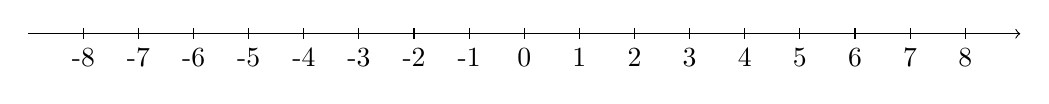
\begin{tikzpicture}[scale=0.7]
  \draw[->] (-9,0) -- (9,0);
  \foreach \x in {-8,..., 8}
    \draw (\x,0.1) -- (\x,-0.1) node[below] {\x};
\end{tikzpicture}
\end{center}
\item  Shade the segment represented by the interval \((-\infty, -6]\) on the number line. Use $\bullet$ to indicate a closed endpoint, and $\circ$ to indicate an open endpoint.
\begin{center}
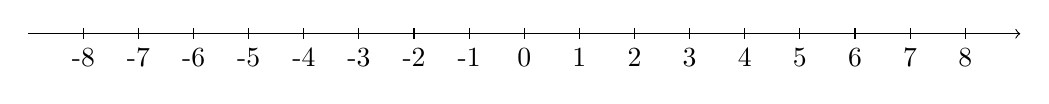
\begin{tikzpicture}[scale=0.7]
  \draw[->] (-9,0) -- (9,0);
  \foreach \x in {-8,..., 8}
    \draw (\x,0.1) -- (\x,-0.1) node[below] {\x};
\end{tikzpicture}
\end{center}
\item The interval represented by the shaded segment below is \rule{10em}{0.1pt} .
\begin{center}
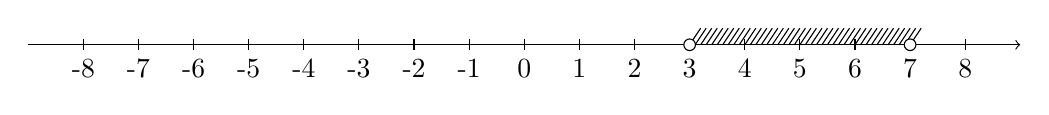
\begin{tikzpicture}[scale=0.7]
  \draw[->] (-9,0) -- (9,0);
  \foreach \x in {-8,..., 8}
    \draw (\x,0.1) -- (\x,-0.1) node[below] {\x};
  \foreach \x in {3,3.1, ..., 7.1}
    \draw (\x, 0) -- (\x+0.2, 0.3);
\draw[fill=white] (3,0) circle(3pt);
\draw[fill=white] (7,0) circle(3pt);
\end{tikzpicture}
\end{center}
\item
The following graph shows the state of an object cooling over time:

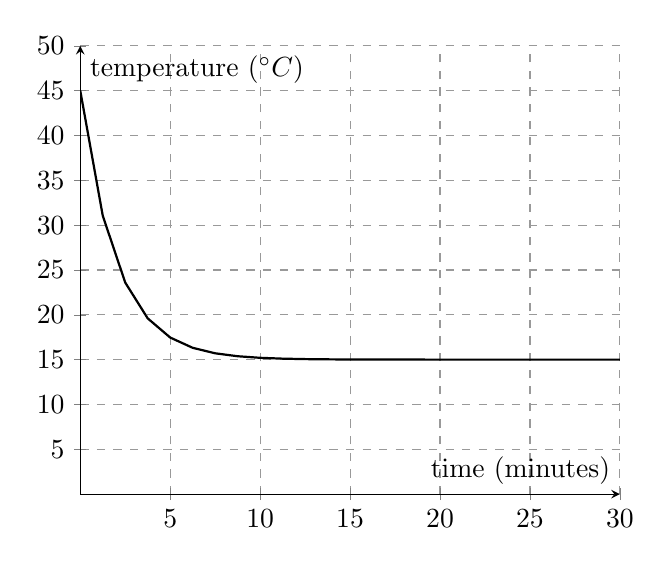
\begin{tikzpicture}
\begin{axis}[
axis lines=middle,
xlabel={time (minutes)},
ylabel={temperature (${}^\circ C$)},
ymin=0, ymax = 50,
domain=0:30,
ytick distance=5,
grid=both,
grid style={draw=gray!80, dashed}
]
\addplot[thick]{15 + 30*e^(-0.5*x) };
\end{axis}
\end{tikzpicture}
\begin{enumerate}
\item 
What is the temperature of the object as time approaches infinity?
\vspace{\stretch{1}}
\item
What can you infer about the room temperature in which this cooling process was taking place?
\vspace{\stretch{1}}
\end{enumerate}
\clearpage
\noindent{\bf Direction.} Describe the end behaviors of the graphs below. If the graph doesn't have a definite end behavior, put ``N/A''.
\item
\begin{center}
\begin{tabular}{cc}
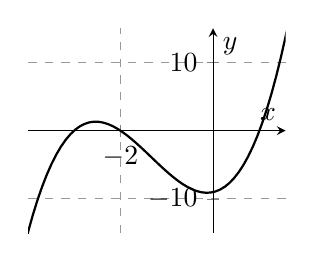
\begin{tikzpicture}[baseline={(current bounding box.center)}]
\begin{axis}[
xlabel={$x$},
ylabel={$y$},
axis lines=middle,
ymin=-15, ymax=15,
domain=-5:5,
samples=100,
width=0.4\textwidth,
grid=both,
grid style={draw=gray!80, dashed}
]
\addplot[thick]{1.5*(x-1)*(x+2)*(x+3)};
\end{axis}
\end{tikzpicture}
&\parbox{0.45\textwidth}{As $x$ approaches $\infty$, $y$ approaches \rule{8em}{.1pt}.\\[1em]
As $x$ approaches $-\infty$, $y$ approaches \rule{8em}{.1pt}.\\[1em]
Does the graph have an absolute maximum?  \rule{4em}{.1pt}.\\[1em]
Does the graph have an absolute minimum?  \rule{4em}{.1pt}.}
\end{tabular}
\end{center}
\vspace{\stretch{1}}
\item
\begin{center}
\begin{tabular}{cc}
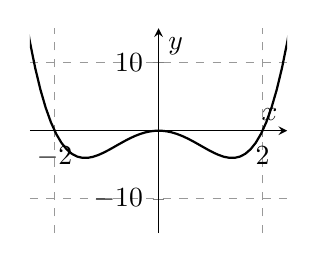
\begin{tikzpicture}[baseline={(current bounding box.center)}]
\begin{axis}[
xlabel={$x$},
ylabel={$y$},
axis lines=middle,
ymin=-15, ymax=15,
domain=-5:5,
samples=100,
width=0.4\textwidth,
grid=both,
grid style={draw=gray!80, dashed}
]
\addplot[thick]{(x-2)*(x+2)*x^2};
\end{axis}
\end{tikzpicture}
&\parbox{0.45\textwidth}{As $x$ approaches $\infty$, $y$ approaches \rule{8em}{.1pt}.\\[1em]
As $x$ approaches $-\infty$, $y$ approaches \rule{8em}{.1pt}.\\[1em]
Does the graph have an absolute maximum?  \rule{4em}{.1pt}.\\[1em]
Does the graph have an absolute minimum?  \rule{4em}{.1pt}.}
\end{tabular}
\end{center}
\vspace{\stretch{1}}
\item
\begin{center}
\begin{tabular}{cc}
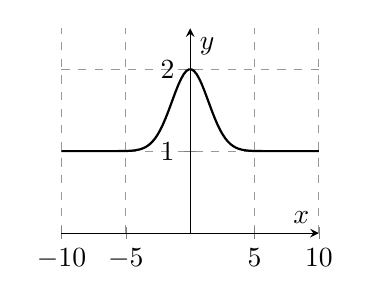
\begin{tikzpicture}[baseline={(current bounding box.center)}]
\begin{axis}[
xlabel={$x$},
ylabel={$y$},
axis lines=middle,
domain=-10:10,
ymax=2.5, ymin=0,
samples=100,
width=0.4\textwidth,
grid=both,
grid style={draw=gray!80, dashed}
]
\addplot[thick]{e^(-x^2/4)+1};
\end{axis}
\end{tikzpicture}
&\parbox{0.45\textwidth}{As $x$ approaches $\infty$, $y$ approaches \rule{8em}{.1pt}.\\[1em]
As $x$ approaches $-\infty$, $y$ approaches \rule{8em}{.1pt}.\\[1em]
Does the graph have an absolute maximum?  \rule{4em}{.1pt}.\\[1em]
Does the graph have an absolute minimum?  \rule{4em}{.1pt}.}
\end{tabular}
\end{center}
\vspace{\stretch{1}}
\item
\begin{center}
\begin{tabular}{cc}
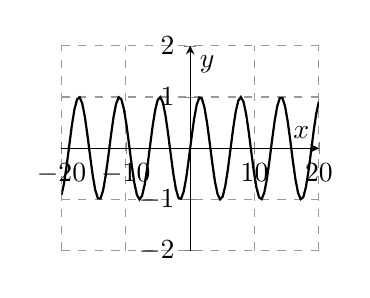
\begin{tikzpicture}[baseline={(current bounding box.center)}]
\begin{axis}[
xlabel={$x$},
ylabel={$y$},
axis lines=middle,
domain=-20:20,
ymax=2, ymin=-2,
samples=100,
width=0.4\textwidth,
grid=both,
grid style={draw=gray!80, dashed}
]
\addplot[thick]{sin(deg(x))};
\end{axis}
\end{tikzpicture}
&\parbox{0.45\textwidth}{As $x$ approaches $\infty$, $y$ approaches \rule{8em}{.1pt}.\\[1em]
As $x$ approaches $-\infty$, $y$ approaches \rule{8em}{.1pt}.\\[1em]
Does the graph have an absolute maximum?  \rule{4em}{.1pt}.\\[1em]
Does the graph have an absolute minimum?  \rule{4em}{.1pt}.}
\end{tabular}
\end{center}
\vspace{\stretch{1}}
\end{enumerate}
\end{document}